%%%%%%%%%%%%%%%%%%%%%%%%%%%%%%%%%%%%%%%%%%%%%%%%%%%%%%%%%%%%%%%%%%%%%%%%%%%%%%
%
% PROJECT PROPOSAL  DESCRIPTION:
%   A concise description of the main concepts of the proposed project.
%
% RESEARCH:
%   A list of research activities which led to this project.
%
% EXPERIMENTS:
%   A list of the experiments performed which supported the research.
%
%%%%%%%%%%%%%%%%%%%%%%%%%%%%%%%%%%%%%%%%%%%%%%%%%%%%%%%%%%%%%%%%%%%%%%%%%%%%%%%
% Define a single space environment (copied from doublespace.sty)
% e.g. \begin{singlespace}
%         single-spaced text
%      \end{singlespace}

\documentclass[12pt,american]{article}
\usepackage{fullpage}
\usepackage{bbm}
\usepackage{url}
\usepackage{subfigure}
\usepackage{babel}
\usepackage{times}
\usepackage{graphicx}
\usepackage{amssymb}
\usepackage{lscape}
\usepackage{verbatim}
\usepackage{enumerate}
\usepackage{afterpage}
\usepackage{setspace}
\usepackage{algorithmic}


\begin{document}
\thispagestyle{empty} 
\begin{center}
{\em MS Thesis Proposal}\\
\vspace{.5in}
{\large \bf Soft-Body Deformations Through Rigid-Body Simulations of Voxelized Meshes Augmented with Bézier Curves}\\
\vspace{.5in}
{\bf James Govan Moir IV}\\
\vfill
\
{\em Committee Chair:} Joe Geigel\\
\vspace{0.1in}
{\em Reader: } Warren R. Carithers\\
 \vspace{0.1in}
Department of Computer Science\\
B. Thomas Golisano College of Computing and Information Sciences \\
Rochester Institute of Technology \\
Rochester, New York \\ [0.3in]
\vspace{0.5in}
\today{}\\
\end{center}
\vfill

%%%%%%%%%%%%%%%%%%%%%%%%%%%%%%%%%%%%%%%%%%%%%%%%%%%%%%%%%%%%%%%%%%%%%%%%%%%%%%%
%%  Collection of useful abbreviations.
\newcommand{\etc} {\emph{etc.\/}}
\newcommand{\etal}{\emph{et~al.\/}}
\newcommand{\eg}  {\emph{e.g.\/}}
\newcommand{\ie}  {\emph{i.e.\/}}
%%%%%%%%%%%%%%%%%%%%%%%%%%%%%%%%%%%%%%%%%%%%%%%%%%%%%%%%%%%%%%%%%%%%%%%%%%%%%%%


%%%%%%%%%%%%%%%%%%%%%%%%%%%%%%%%%%%%%%%%%%%%%%%%%%%%%%%%%%%%%%%%%%%%%%%%%%%%%%%
% Abstract
\section*{Abstract}

The field of soft-body deformations has existed since the 1980's. Due to limitations of the time,
simulation of soft-body deformations couldn't be performed in real-time. As a result, it was only 
suitable for tasks that could be done offline, such as animation. However, with the advent of 
modern computing hardware and advances in soft-body deformation research real-time speeds are now
possible. These advances have made soft-body deformations more appealing to tasks such as surgery 
simulation and video games.

This proposal discusses a technique for soft-body deformations based on voxelized meshes, a brief
background of research done in the field, a proposed extension to the voxelized mesh technique, a 
hypothesis on how the extension will fare against the existing technique, and the design of a system
that will be used to compare the proposed extension and the original technique.

% This should be a short description of the work and the results: a paragraph 
% or two summarizing your project proposal. Note that an abstract is meant to be read 
% independently from the rest of the project report so you cannot cite your 
% paper or other papers in it. It would be useful to examine other abstracts 
% in the many papers you have read to understand what an abstract really is.
%%%%%%%%%%%%%%%%%%%%%%%%%%%%%%%%%%%%%%%%%%%%%%%%%%%%%%%%%%%%%%%%%%%%%%%%%%%%%%%
\vfill{}

%%%%%%%%%%%%%%%%%%%%%%%%%%%%%%%%%%%%%%%%%%%%%%%%%%%%%%%%%%%%%%%%%%%%%%%%%%%%%%%
% This is where the main body of the capstone proposal starts
\setcounter{page}{0} 
\newpage{}

\section{Introduction}
% This part of the proposal should be a couple of paragraphs that
% describe the reason for your proposal and your project/thesis area at
% high level.

Research in the field of soft-body deformation simulation has been ongoing since the 1980's, 
originating with the seminal paper by Terzopoulos \etal, Elastically Deformable Models 
\cite{Elastically-Deformable-Models}. Since then, the field has 
grown to encompass several areas of research for achieving realistic soft-body deformations. These
areas include Mass-Spring systems and Finite Element Method systems. 
% TODO: reference mass-spring and fem papers
These systems are typically used in animation, surgery simulation, and video games.

Due to the limitations at the time, solutions for performing soft-body deformations typically didn't
operate at real-time speeds. These limitations aren't as apparent in systems that don't operate at
real-time speeds, such as animation systems. However, systems such as surgery simulators and video
games must operate at real-time speeds. So it's vital that any soft-body deformation simulation that
they make use of are as fast as possible. With research into new techniques and the advent of modern
hardware, solutions which operate in real-time have come into existence. Some examples of solutions 
which achieved real-time speeds
are Stable Real-Time Deformations \cite{Stable-Real-Time-Deformations} and Deformable Object 
Simulation in Virtual Environment \cite{Deformable-Object-Simulation-in-Virtual-Environment}.

Another solution which took a different approach was described in the work done by Müller \etal 
Their solution was able to perform motion, deformation, and fracture 
simulations in real-time. To achieve this, Müller \etal utilized a voxelized representation of 
meshes, or voxel-meshes, generated at run time \cite{Muller_Teschner_Gross}. These voxel-meshes 
contained references
to the mesh used to create them, so that when a voxel  was modified by some force the portion of 
the mesh that it referenced was also modified. The forces for deformation and motion were calculated 
using rigid-body physics, while the forces for fracturing were calculated using the finite element 
method. However, the described solution does have some draw backs. The voxelization of meshes at run
time can be costly, especially for models with a high vertex count. Also, a higher voxelization 
count would be required to improve upon the accuracy of deformations for a specific object. 

The remainder of this proposal focuses on a new technique which aims to improve upon the work
done by Müller \etal by combating the previously mentioned drawbacks. To achieve this, the proposed
technique will make use of 
Bézier curves and deformable voxels. The Bézier curves will be used to control the positions of the
mesh's vertices and the control points of the Bézier curves will be placed on the hull of the voxels.
The deformable voxels will allow these control points to move, resulting in the deformation of the 
mesh. In theory, this will result deformations which are less expensive to compute and are more 
accurate.
%TODO: add a paragraph explaining my extension to muller

\section{Background}
% This section should be sufficient for the reader to understand the
% project area and the relevance of your efforts in the world of
% computer science. The description here should be provide the
% motivation to the reader that you are exploring a problem area that is
% relevant to the CS community.

The field of soft-body deformations has been around since the 1980's, originating with Terzopoulos
\etal's seminal paper Elastically Deformable Models \cite{Elastically-Deformable-Models}. Since 
then, an extraordinary amount of work has been done in the field of soft-body deformations. A 
non-comprehensive overview of this work can be seen in the surveys done by Frisken \etal 
\cite{A-Survey-of-Deformable-Modeling-in-Computer-Graphics} and Nealen \etal
\cite{Phyiscally-Based-Deformable-Models-in-Computer-Graphics}.
We'll observe some of the work done in this field, mainly for deformations of solid 
three-dimensional objects, for two types of systems. Systems based on the Finite Element Method 
(FEM) and Mass-Spring systems. 

\subsection{FEM Systems}

The Finite Element Method works by taking an object and subdividing it into a collection of shapes.
Typically, tetrahedral subdivisions are used for 3D objects, although others can be used as well.
Each object which constitutes the subdivision is made up of a series of points, refereed to as nodes.
These nodes are used to construct matrix, one for each object. These matrices are then combined 
based on neighboring nodes to create what is refereed to as the stiffness matrix. The stiffness 
matrix is used to determine how the object reacts to applied forces \cite{FEM-Explenation}.

The earliest application of FEM to soft-body deformations was in the work done by Terzopoulos \etal
\cite{Elastically-Deformable-Models}. Their work was based on previous work in modeling and 
elastic theory. FEM was used to discretize the equations of motion, with 
focus on surfaces, to achieve their deformations. This yielded realistic results for a number of 
simple objects. 
%TODO: add overview of FEM

FEM systems can be used to achieve fairly realistic deformations. However, the calculations that 
need to be done are fairly expensive, so achieving real-time deformations is difficult. Although,
work has been done to improve the performance of this technique.
An early instance of this method achieving near real-time performance was with the work done by 
Witkin et al. \cite{Fast-Animation-and-Control-of-Nonrigid-Structures}. In their work, deformable 
models were constructed from non-rigid pieces using point-to-point attachment constraints. 
%(NEED TO RE-READ THIS)

A method for fast physically accurate simulation for real time animation and interaction was 
introduced in the work done by James \etal \cite{ArtDefo-Accurate-Real-Time}. 
Unlike previously discussed papers, they used a combination of boundary 
integrals and the boundary element method. To achieve real-time performance, values which are 
typically too expensive to calculate at run time are pre computed and stored in a database for 
lookup during run-time. This lead to the performance of a real-time simulation, at the cost of 
memory and the need to pre-compute values.

Another method for real-time simulation using FEM was introduced in the work done by Debunne \etal 
\cite{Dynamic-Real-Time-Deformations-Using} 
using space and time adaptive sampling. In their work, they describe a system which makes use of a 
non-nested multi-resolution tetrahedral mesh. As objects are deformed in their simulation the 
tetrahedral mesh is refined to focus computation on areas with more deformations than others. This 
level of detail system ensured that meshes don’t become too coarse during deformation. They also 
applied this technique to mass-spring systems. However, it was found that this leads to less 
accurate results.


\subsection{Mass-Spring Systems}

%TODO: add overview of mass-spring systems

Mass-Spring systems treat objects as a network of mass-nodes and springs. As the name implies, 
mass-nodes are points with a specified mass. These nodes are connected to other nodes in the object
with a number of springs. These springs are typically treated as ideal weightless springs. The 
configuration of these springs can vary depending on the desired effect. 
% An illustration of this 
% hierarchy can be seen in Figure \ref{}.
Once the mass-nodes and 
spring network is configured, physical interactions can easily and quickly be simulated by applying
hooke's law, \(F_s = kx\), to each node. 

Mass-Spring systems usually make use of several types of springs to create their deformations. For
instance, in the work done by Chen \etal \cite{Physically-Based-Animation-of-Volumetric-Objects} a
combination of structural, shear, and flexion springs are used. Structural springs are used to
simulate deformations that occur under compressive forces, shear springs are used to simulate shear
forces, and flexion springs are used to simulate flexion deformations. %TODO: re-word
These springs are connected to mass-nodes and the stretching and compression of theses springs 
creates the deformations. For the case of this appear, the mass nodes are connected in a voxel 
structure. As forces are applied to the structure, these connections persist, allowing deformations
to correctly propagate across voxels. However, as a drawback the object has to be rendered as a 
series of voxels. The work done by chen \etal was able to run at interactive speeds.

The introduction of general-purpose computing on graphics processing units (GPGPU) presented a way 
to easily improve the performance of Mass-Spring systems. The work provided by Chang \etal 
\cite{Deformable-Object-Simulation-in-Virtual-Environment} 
 introduced a method for computing deformations 
with a mass-spring model on the GPU. The calculations and subsequent rendering of the deformations 
are done in the vertex and fragment shaders. In order to store the velocity, position, and 
connectivity data on the GPU a series of textures are used, two for each data type. This texture 
duplication allows them to overcome the difficulty of not being able to read and write to the same 
texture. This technique also allows them to keep all of the deformation calculations on the GPU 
without the need to send information back to main memory, which is a considerable bottle-neck. Their 
implementation resulted in a simulation which ran in real-time for objects with over 170,000 
springs.

An important part in creating realistic deformations is volume preservation. Volume preservation is 
normally something which is fairly expensive to compute. Vassilev \etal 
\cite{Simulation-of-a-Deformable-Human-Body} 
 attempts to achieve this by introducing a new type of spring, the support spring, to simulate the 
matter within an object. These springs are connected perpendicular to surface vertices with equal 
length. They are also connected to an imaginary frame within the body. These springs then combat any 
compressive forces that might result in inaccurate volume changes. Their approach achieved real-time 
speeds for meshes of approximately 7000 triangles. 

\subsection{Physically-Based Simulation of Objects Represented by Surface Meshes}
%TODO: add sub-section for muller's paper and it's shortcomings

The paper by Müller \etal describes a system which utilizes voxelized meshes for deformation and
fracturing. The described system generates voxels at run time. These voxels are augmented with 
several attributes for use in simulation, which can be seen in tables 
\ref{tab:CubeElementAttributes} and \ref{tab:VertexAttributes}. 
These attributes are used both for applying 
deformations to the mesh and for performing the necessary physics simulation. The physics simulation 
necessary for animation of the mesh can be implemented using FEM or with a rigid body physics 
simulation. Although, the implementation described in the paper utilizes a FEM system. A FEM
system is also used to calculate the forces for simulating surface fracture. During simulation, the 
positions of the voxels are modified. These changes in position are then
applied to the triangles contained by the effected voxels. Resulting in surface deformations. The 
resulting simulation was able to produce deformations and fractures of meshes consisting of 23,000 
triangles and an equivalent voxelized representation of 800 voxels at a rate of 10 to 15 frames per
second.

The described system does come with some draw backs. For instance, the voxelization of meshes at
run time is a somewhat costly for complex models and unnecessary step. Furthermore, in order to 
improve the accuracy of deformations a higher voxelization count would be needed, which would 
negatively impact performance. 


\begin{table}
  
\begin{center}
 \begin{tabular}{|c | c|} 
 \hline
 Attributes & Description \\ [0.5ex] 
 \hline\hline
 \(x, y, z\)& Integer position indices with respect to the bounding box of the surface  \\ 
 \hline
 \(v[8]\) & Pointers to vertices  \\
 \hline
 triangles & Pointer to the list of triangles that intersect the element\\
 \hline
\end{tabular}
\end{center}

\caption{Cube element attributes described in Müller \etal}\label{tab:CubeElementAttributes}
\end{table}

\begin{table}
  \begin{center}
    \begin{tabular}{|c | c|} 
      \hline
      Attributes & Description \\ [0.5ex] 
      \hline\hline
      position & Position in the deformed mesh  \\ 
      \hline
      velocity & Velocity for dynamic simulations  \\
      \hline
      mass & Mass lumped from all adjacent cubes\\
      \hline
    \end{tabular}
  \end{center}
  
  \caption{Vertex attributes described in Müller \etal}\label{tab:VertexAttributes}
\end{table}

%TODO: rename to solution and give a more in depth/high level description of the changes i would make
%TODO: add pseudo code here
%TODO: for the hypothesis specificly mention the metrics i'll be measuring
\section{Solution}
% TODO: come back to this, better describe the extension and my thoughts behind it.
To improve upon the work done by Müller \etal, I propose the following additions. Bézier curves 
should be constructed from mesh edges contained within each voxel and the voxels should be 
deformable.

The Bézier curves will be the main source of deformations. They will be constructed from the edges
of the underlying mesh during voxelization. To construct a Bézier curve, a ray will be cast along 
the corresponding edge of the underlying mesh. The intersections between this ray and the voxel will
be the first and last control points for the Bézier curve. The remaining control points will use the
edge's starting and ending points if the whole edge is contained by the voxel. Otherwise, the vertex
contained by the voxel will be the only control point. The resulting Bézier curve will either be a
quadratic or a cubic curve. In order for this Bézier curve to correctly reconstruct the edge that it
was constructed from, the point on the curve that corresponds to the edge's start and end points 
needs to be found. For quadratic Bezier curves, this can be done by taking the original formula and
rewriting it from the form:

\[P = (1 - t)^2P_0 + 2(1 - t)tP_1 + t^2 P_2\]

\begin{center}
To:
\end{center}
  
\[0 = (P_0 - 2P_1 + P_2)t^2 + (-2P_0 + 2P_1)t + (P_0 - P)\]

The quadratic equation can then be used to solve for \(t\). For cubic Bézier curves, the same 
process can be done. First, the equation for the cubic Bézier curve is rewritten from:

\[P = (1 - t)^3P_0 + 3(1 - t)^2tP_1 + 3(1 - t)t^2P_2 + T^3P_3\]

\begin{center}
To:
\end{center}

\[0 = (-P_0 + 3P_1 - 3P_2 + P_3)t^3 + (3P_0 - 6P_1 + 3P_2)t^2 + (-3P_0 + 3P_1)t + (P_0 - P)\]

Then, the cubic equation can be used to solve for the two \(t\) values needed, one for each 
endpoint. The pseudo code that describes the construction of the voxels and Bézier curves can be 
seen in Figure \ref{fig:VoxelizationAlgorithm}.

In order for the shape of the Bézier curves to change their control points must be moved somehow.
The addition of deformable voxels allows this to occur. As voxels are deformed, the control points
which are attached to the hull will be adjusted based on the voxel deformation. A simplified 
two-dimensional example can be seen in Figure \ref{fig:Extension2DExample}. Here we see the direction 
which force is 
applied to the voxel and the resulting voxel deformation. We also see how the deformation modifies
the position of the control point, the resulting change in the Bézier curve, and the modified 
position of the vertices.

\begin{figure}[h]
  \centering
  \includegraphics{Extension2DExample}
  \caption{Deformation example in 2D}
  \label{fig:Extension2DExample}
\end{figure}

% Bezier curves
% shall be constructed using the edges contained within each voxel and their starting and ending
% control points will be placed on the internal faces of the voxel. Second, the voxels will be 
% allowed to deform based on forces applied to each voxel face. These deformations will cause the 
% control points of the Bezier curves to move, resulting in their shape being modified. This shape
% modification will then be used to modify the mesh, creating the deformation.

My hypothesis is that the proposed extension will provide soft-body deformations that are more
realistic to the human eye and more efficient to compute, leading to a higher frame rate, than the 
original technique. In theory, the use of the
Bezier curves and deformable voxels should allow for a low resolution voxel-mesh to achieve similar
deformations to that of a high resolution voxel-mesh.

\begin{figure}
  \hrule
  \vspace{6pt}
  \begin{algorithmic}
  \REQUIRE $size$, The size of the voxels
  \REQUIRE $hollow$, Specifies if the resulting voxel-mesh should be hollow
  \STATE Create a bounding box using the mesh's minimum and maximum vertex
  \STATE Populate the bounding box with voxels of uniform size specified by $size$
  \STATE Place each triangle of the mesh into a tight bounding box
  \FOR{For each Voxel $v$}
      \IF{If $v$ intersects a triangle's bounding } 
          \STATE save $v$
      \ENDIF
  \ENDFOR
  \IF{$hollow$ is true}
      \FOR{For each 2D slice of the bounding box}
          \STATE Fill the voxels that are contained within the existing voxels
      \ENDFOR
  \ENDIF
  \FOR{For each Voxel $v$}
      \FOR{For each edge $e$ in $v$}
          \STATE Cast a ray along $e$ in the directions of its starting and end points
          \STATE Use the intersection points as the first and last control points of the Bézier curve for this edge
          \STATE Use the endpoints of $e$ that are contained by $v$ as the remaining control point(s)
          \STATE Calculate the position on the Bézier curve that corresponds to the endpoints of $e$ that are contained by $v$
      \ENDFOR
  \ENDFOR
  \RETURN the voxel-mesh
  \end{algorithmic}
  \hrule
  \vspace{6pt}
  \caption{Voxelization Algorithm Pseudo Code}
 \label{fig:VoxelizationAlgorithm}
\end{figure}

% Summarize what you think the problem is, and what your hypothesis
% is. Here is a small example based on a successful project by Priyanka
% Sinha: ''Using one technique for schema matching does not seem
% adequate. The hypothesis underlying this sproject is that a holistic
% approach to schema matching based on the three techniques described
% earlier would do an effective approach to schema matching.''

% Additional description to circumscribe the work so that the reader
% knows what you plan to do to establish your hypothesis.

% \section{Solution Design and Implementation}
% Describe how you plan to design and implement a solution. 

% You must also describe how you would use your solution to establish the validity of your hypothesis. 
% Explain the measurements you plan to conduct and how these would establish the validity 
% (or invalidity) of your hypothesis.

%TODO: rename to implementation
\section{Implementation}
\subsection{Hypothesis Validation}

To Validate the claims made in the hypothesis, the original technique described by Müller \etal and
the proposed extension will need to be implemented. These implementations will then be used to 
collect data for evaluating the hypothesis.

\subsection{Design}

The original technique and the proposed extensions will be implemented as two applications. The 
first application will be used to generate the voxel-meshes that are needed by both techniques. The
second application will perform the physics simulation. This approach was chosen to remove the need
for voxelization, which can be a costly operation when implemented in a naive fashion, to occur at
simulation run time.

\subsection{Libraries and APIs}

Both applications will make use of a number of libraries and APIs to achieve their respective goals. 
The following is a comprehensive list of the libraries that will be used:

% TODO: links
\begin{itemize}
  \item Bullet Physics: An open source physics engine.
  \item OpenGL: The Open Graphics Library.
  \item GLM: A math library compatible with GLSL math functions.
  \item GLAD: An OpenGL extension loader.
  \item nlohmann/json.hpp: An open source json library for C++.
  \item Dear ImGui: A simple to use, immediate-mode GUI library.
\end{itemize}

\subsection{Voxelization Application Design}

The voxelization application will require the following components: A simple GUI, a mesh loader,
a voxelizer, a renderer, and a voxel-mesh serializer. The renderer and voxel-mesh serializer will 
be provided by the shared library, which is discussed in section \ref{SharedLibrary}. 

The simple GUI would allow a user to select a mesh to voxelize, specify some parameters for the 
voxelizer, and specify a location to save the resulting voxel-mesh. Since the needs of the GUI are 
so simple, a complex GUI library won't be needed. So the Dear ImGui library will suffice.
% TODO: consider including the mock-up used in the independent study?

The mesh loader would need to convert the contents of a specified file into a mesh usable by the
application. Since there already exists many file formats for the exporting and importing of meshes
produced by 3D modeling applications, a custom format won't be used. Preferably, the file format 
would be simple to reduce the complexity of the design and implementation of the mesh loader. As
such, the Wavefront OBJ file format will be used, since it meets the previously stated criteria.

The voxelizer should take a mesh, loaded by the mesh loader, and convert it into a voxel-mesh. To
achieve this, a naive voxelization algorithm will be used. Since the voxels also need to contain
information for the Bezier curves, it will also generate this information. The pseudo code for the 
proposed voxelization algorithm can be seen in figure \ref{fig:VoxelizationAlgorithm}.

% TODO talk about renderer and serializer


\subsection{Physics Simulation Application Design}

The physics simulation application will require the following components: a GUI, a physics 
engine, a renderer, a voxel-mesh manager, a voxel-mesh deserializer, and a scene serializer. The 
renderer and voxel-mesh deserializer will be provided by the shared library.

%TODO: make this not indent
The GUI should allow the following:

\begin{itemize}
  \item The loading of voxel-meshes.
  \item The selection of loaded voxel-meshes.
  \item The modification of voxel-mesh settings, for use in the physics simulation.
  \item The specification of initial forces to be applied to voxel-meshes during physics simulation.
  \item The general settings of the physics simulation.
  \item Whether the proposed extension is enabled or disabled.
  \item The ability to start, stop, and reset the simulation.
  \item The saving of a scene's layout, physics settings, and voxel-mesh settings for later use and
  experimentation.
\end{itemize}

In order to support the loading and management of numerous voxel-meshes a voxel-mesh manager is 
needed. The voxel-mesh manager will handle all data needed to render the voxel-meshes, perform
deformations, and run the physics simulation. This data includes the voxel-mesh data structure and
the physical data for the voxel-meshes. The voxel-mesh manager will accept voxel-meshes and return a 
handle to the application for accessing the voxel-meshes at later times. 
To handle data storage, the voxel-mesh manager will make use of use a series of key-value pairs. To 
support the ability to reset the physics simulation, the voxel-mesh manager will also store a
copy of the original voxel-mesh before any deformation has been applied and the original physical 
information.

Rather than design, implement, and test a custom physics engine, an existing physics engine will be
used. With this in mind, the physics simulator is designed to wrap an existing physics engine 
implementation. The design provides a simple interface to the underlying physics implementation. To 
add objects to the physics simulation, a handle to a voxel-mesh is passed to the interface. The 
underlying implementation would then use this handle to retrieve any information that it needs to 
setup the object for simulation. 

\subsection{Shared Library Design} \label{SharedLibrary}

Due to the fact that a significant amount of functionality is shared between the Voxelization
application and the Physics Simulation application, a shared library will be used. This shared
library will contain the necessary implementations and interfaces needed by the two applications. 
The contents of this library in relation to its use by the applications can be seen in figure
\ref{fig:SharedLibraryUML}.

\begin{figure}[h]
  \centering
  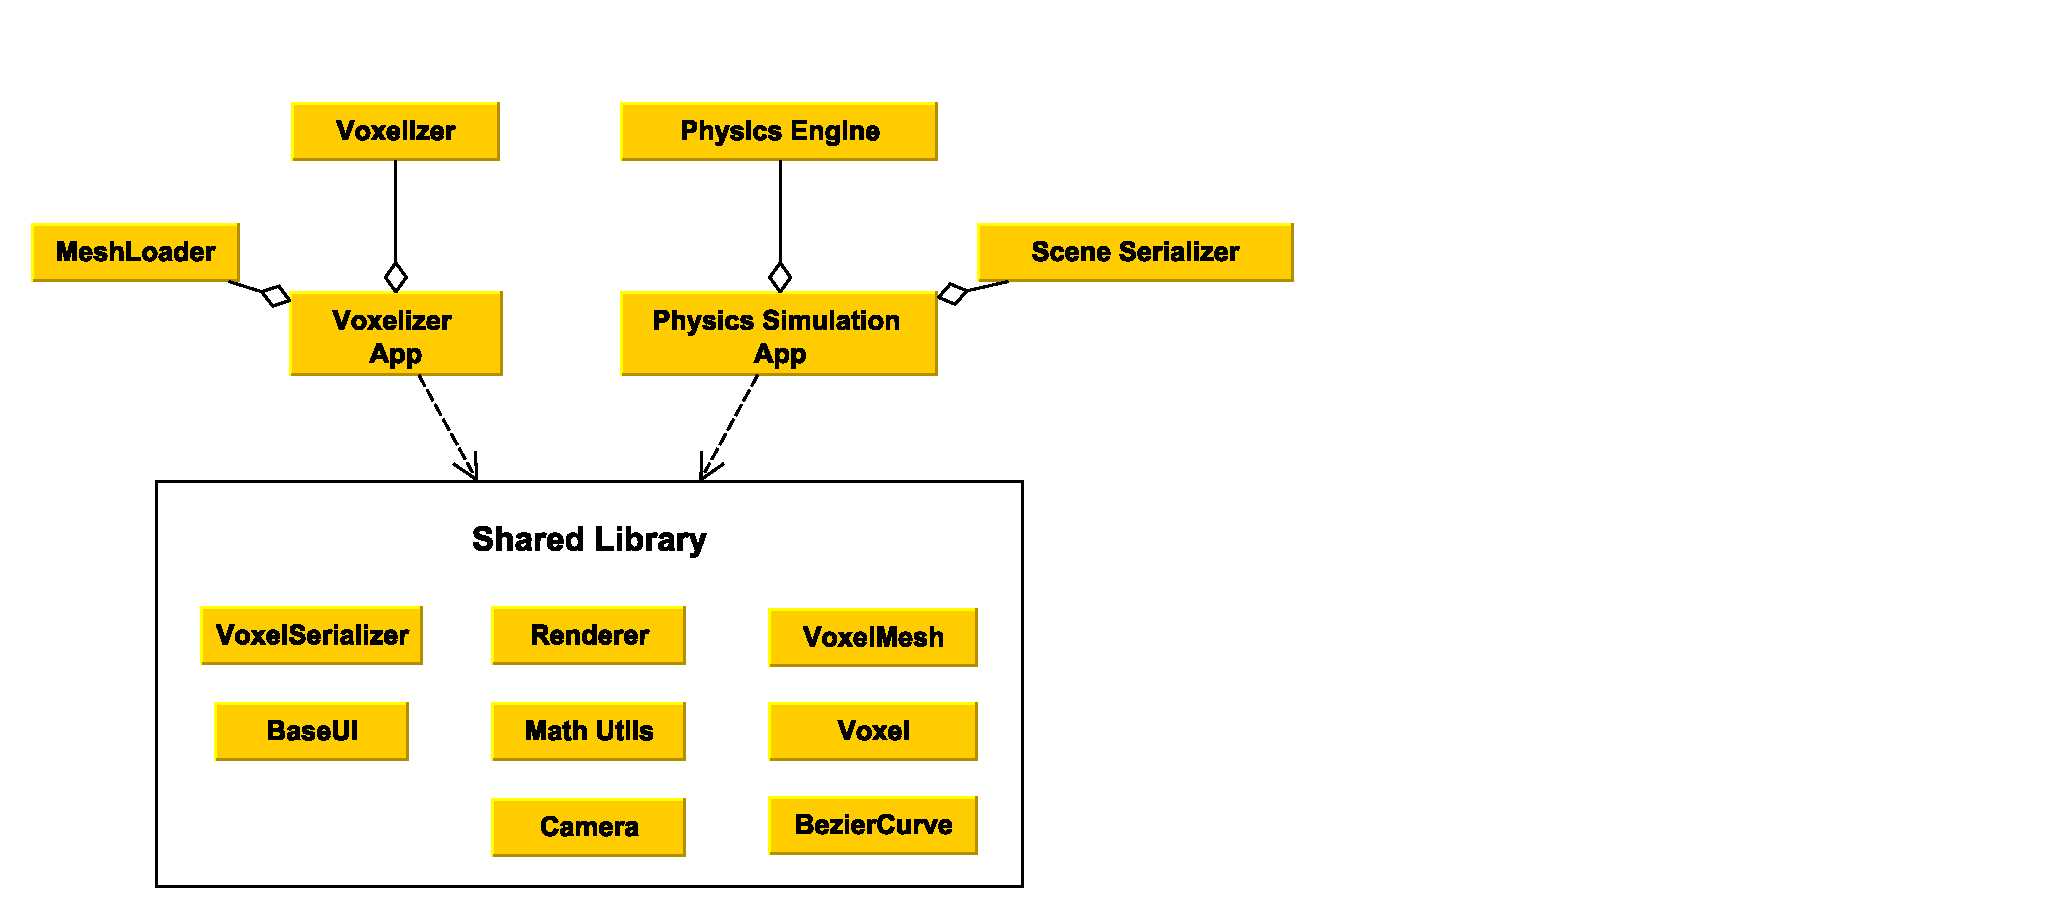
\includegraphics[width=0.8\textwidth, trim={0cm 0cm 15cm 0cm}]{SharedLibraryUML}
  \caption{Shared Library UML Diagram}
  \label{fig:SharedLibraryUML}
\end{figure}

\subsubsection{Voxel-Mesh Serializer}
The voxel-mesh serialization and deserialization will be handled by a single class. This class will
manage the resources of the file containing the serialized voxel-mesh. 
This class will also utilize the nlohmann/json.hpp library for serializing to JSON.
% the underlying serialization library, which will be discussed in section \ref{Serialization}. 
Since this class handles both serialization and deserialization, it's possible to overwrite the 
contents of a file by mistake. To remedy this, on construction the class will take in a parameter to 
specify if its read-write permissions. 

\subsubsection{Renderer}
% Renderer

The renderer will consist of two classes, one to act as a frontend and the other to act as a
backend. The frontend will manage all resources associated with the scene. This includes the 
tracking of what objects are in the scene, their positions, and their various physical attributes.
The frontend will also provide a collection of methods to add and remove objects to the scene and to 
draw the current scene. These methods will convert the scene into a collection of handles which the
backend will use to draw the scene.

The backend will manage all resources used by OpenGL. To achieve this, a series of caches will be 
used. These caches will consist of key-value pairs, where the key is some generated integer and the
value is what data the cache is managing. These caches will be used to manage vertex data, textures,
and shader programs. The backend will also handle all OpenGL state and function calls.

\subsubsection{Base UI}
% Base UI

Since both applications will be using the same GUI library, it makes sense for a common interface
to be designed. This interface will handle the initialization and de-initialization of the library.
The interface will also provide methods for retrieving and setting information for the GUI. The
GUIs implemented by the Voxelization and Physics Simulation applications will inherit from this
interface and implement the specific layout of the GUI that meets their needs.

% Math Utils
\subsubsection{Math Utils}

The physics engine that will be used provides their own math library. However, the two applications
will make use of a different math library. So, to reduce the difficulties of needing to constantly
convert from data structures used by one library to the other a collection of conversion functions
will be used. 

\subsubsection{Camera}
% Camera

Both applications will need a camera which can easily be moved around based on inputs by the user.
A single class will be used to fit these needs. This class will manage the position and rotation
of the camera. This class will also provide a method to generate the camera matrix for use by the
renderer. Several methods will be provided to allow the camera's position to be modified by 
providing a new position vector or by providing a velocity vector. Methods will also be provided for
modifying the rotation of the camera by providing rotation matrices or vectors encoding euler angles.

% Voxel objects
\subsubsection{Voxel objects} \label{VoxelObjects}

Some data structures used in voxelization and deformation will be shared between the applications.
These include the Bezier curve, Voxel, and the voxel-mesh. The Bezier curve structure will contain
the control points that define the curve and the values along the curve that can be used to 
calculate the position of the vertex that they control. This structure also provides methods for
calculating the position of this vertex. The Voxel structure contains a list of Bezier curves, a 
list of vertices, a position, a delta position, and its position relative to the center of the 
voxel-mesh that contains it. The voxel-mesh contains a mesh object, the extents of the voxel-mesh 
in voxel space, the size of the voxel-mesh in object space, and a map which contains the voxels and
uses their position in voxel space as the key.

% \subsection{Serialization Design} \label{Serialization}

% In order to support serialization of data structures a serialization format must be selected. 
% Ideally, this format should well documented, have pre-existing libraries that use it, and should
% be human readable. With these in mind, it was decided to use the JSON format for serialization. It
% was also decided to use nlohmann/json.hpp library, as this library provides many useful features 
% that are ideal.

\section{Data Collection}
%TODO: add table for all the data i'll be collecting

Two important data sets will need to be collected in order to validate the claims made in the 
hypothesis: performance data and visual evaluation data. Performance data will need to be collected
from an implementation of the technique described by Müller \etal The visual evaluation data will
need to be collected from an online user study.

\subsection{Performance Data Collection}

A number of metrics will be collected in order to evaluate the performance claims made in the
hypothesis. A list of these metrics can be 
seen in Table \ref{tab:TimingEvaluationMetrics}. The average frame rate will be 
used to directly evaluate and compare the performance of the two implementations, as the 
performance of the techniques will directly affect the frame rate. The average vertices and Bézier 
curves per voxel will be used to further evaluate the effectiveness of the proposed extension.

\begin{table}
  \begin{center}
    \begin{tabular}{|c|} 
      \hline
      % Metric & Description \\ [0.5ex] 
      % \hline\hline
      Avg. Frame Rate  \\ 
      \hline
      Avg. Vertices per voxel   \\
      \hline
      Avg. number of Bézier curves per voxel \\
      \hline
    \end{tabular}
  \end{center}
  
  \caption{Timing evaluation metrics}\label{tab:TimingEvaluationMetrics}
\end{table}


\subsection{Visual Evaluation Data Collection}

% this needs to be re-worded a bit
The visual evaluation data will be collected through an online user study, with a sample size of
20 to 25 users. The study will present users with two side-by-side videos. The videos will present 
the user with recordings of the same deformation setup, but one side will showcase the deformations 
produced by the original technique, while the other side will showcase the deformations produced by 
the proposed extension. The sides in which the two videos appear will be randomized. The study will 
ask the user to evaluate the realism of the deformations on a scale of one to ten. In order for this
study to take place IRB approval will be required.

\section{Roadmap}
The following is a tentative schedule for the completion of this thesis:
\begin{itemize}
  \item End of May: Both applications will be completed.
  \item End of June: Data will be collected for the evaluation. First draft of thesis will be 
  completed.
  \item End of July: Second draft and final draft of the thesis will be completed.
  \item Beginning of August: Thesis defense.
\end{itemize}

% Here you need to describe your project plan, with dates and deliverables. 

% You must review the CS graduate handbook for details, and yes, make
% sure you also address all of the handbook's requirements for a
% proposal.

%%%%%%%%%%%%%%%%%%%%%%%%%%%%%%%%%%%%%%%%%%%%%%%%%%%%%%%%%%%%%%%%%%%%%%%%%%%%%%%

%%%%%%%%%%%%%%%%%%%%%%%%%%%%%%%%%%%%%%%%%%%%%%%%%%%%%%%%%%%%%%%%%%%%%%%%%%%%%%%
\bibliographystyle{plain}
% Single space the bibliography to save space.
\singlespacing
\bibliography{bibliography}
%%%%%%%%%%%%%%%%%%%%%%%%%%%%%%%%%%%%%%%%%%%%%%%%%%%%%%%%%%%%%%%%%%%%%%%%%%%%%%%


\end{document}
